\documentclass[compress]{beamer}
\usepackage{ifthen,verbatim}

\newcommand{\isnote}{}
\xdefinecolor{lightyellow}{rgb}{1.,1.,0.25}
\xdefinecolor{darkblue}{rgb}{0.1,0.1,0.7}

%% Uncomment this to get annotations
%% \def\notes{\addtocounter{page}{-1}
%%            \renewcommand{\isnote}{*}
%% 	   \beamertemplateshadingbackground{lightyellow}{white}
%%            \begin{frame}
%%            \frametitle{Notes for the previous page (page \insertpagenumber)}
%%            \itemize}
%% \def\endnotes{\enditemize
%% 	      \end{frame}
%%               \beamertemplateshadingbackground{white}{white}
%%               \renewcommand{\isnote}{}}

%% Uncomment this to not get annotations
\def\notes{\comment}
\def\endnotes{\endcomment}

\setbeamertemplate{navigation symbols}{}
\setbeamertemplate{headline}{\mbox{ } \hfill
\begin{minipage}{5.5 cm}
\vspace{-0.75 cm} \small
\end{minipage} \hfill
\begin{minipage}{4.5 cm}
\vspace{-0.75 cm} \small
\begin{flushright}
\ifthenelse{\equal{\insertpagenumber}{1}}{}{Jim Pivarski \hspace{0.2 cm} \insertpagenumber\isnote/\pageref{numpages}}
\end{flushright}
\end{minipage}\mbox{\hspace{0.2 cm}}\includegraphics[height=1 cm]{../cmslogo} \hspace{0.1 cm} \includegraphics[height=1 cm]{../tamulogo} \hspace{0.01 cm} \vspace{-1.05 cm}}

\begin{document}
\begin{frame}
\vfill
\begin{center}
\textcolor{darkblue}{\Large Toy MC model of supersector geometry}

\vfill
\begin{columns}
\column{0.3\linewidth}
\begin{center}
\large
Jim Pivarski
\end{center}
\end{columns}

\begin{columns}
\column{0.3\linewidth}
\begin{center}
\scriptsize
{\it Texas A\&M University}
\end{center}
\end{columns}

\vfill
 9 July, 2010

\end{center}
\end{frame}

%% \begin{notes}
%% \item This is the annotated version of my talk.
%% \item If you want the version that I am presenting, download the one
%% labeled ``slides'' on Indico (or just ignore these yellow pages).
%% \item The annotated version is provided for extra detail and a written
%% record of comments that I intend to make orally.
%% \item Yellow notes refer to the content on the {\it previous} page.
%% \item All other slides are identical for the two versions.
%% \end{notes}

\small

\begin{frame}
\frametitle{Motivation}
\begin{itemize}
\item This ``supersector rotation'' model that we've been talking about is hard to visualize
\item I wanted to make sure that I was thinking correctly about it, e.g.\
deriving the right conclusions about local $x$ and $y$ residuals
\end{itemize}

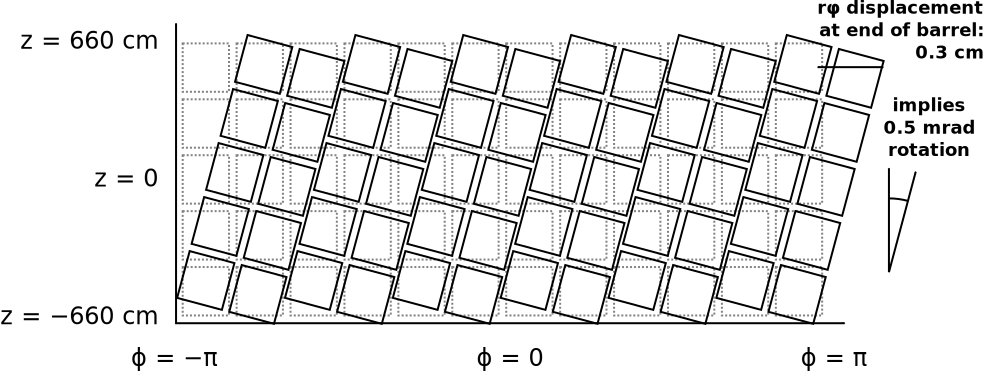
\includegraphics[height=2.7 cm]{just_model2.pdf} \includegraphics[height=2.7 cm]{with_twist.png}

\vspace{0.25 cm}
\hspace{-0.83 cm} \textcolor{darkblue}{\large Toy MC}
\begin{itemize}
\item Built a simple model of rigid-body supersectors in Python/ROOT
\item Applied a supersector rotation (confirmed quantitative predictions)
\item Searched for weak modes
\begin{itemize}
\item it turns out that this is a fairly simple system; easy to diagnose
\end{itemize}
\end{itemize}
\end{frame}

\begin{frame}
\frametitle{Toy MC}
\begin{columns}
\column{0.6\linewidth}
\begin{itemize}
\item Consists of six planes
\begin{itemize}
\item perpendicular to rays from the beamline ($x=0$, $y=0$)
\item distance $R$ from beamline
\item widths = $R\tan\left(\frac{2\pi}{6}\right)$, so that they just touch
\end{itemize}
\item Apply rotations, translations to test deformations
\item Monitor distance between control points along edges (without any deformation, this \mbox{distance is exactly zero)\hspace{-5 cm}}
\begin{itemize}
\item \mbox{example with an exaggerated supersector rotation applied:\hspace{-5 cm}}
\end{itemize}
\end{itemize}

\column{0.4\linewidth}
\includegraphics[width=\linewidth]{model_ideal.pdf}

\vspace{1 cm}
\end{columns}
\vspace{0.2 cm}
\includegraphics[width=0.2\linewidth]{model_whp2.pdf}
\includegraphics[width=0.2\linewidth]{model_whp1.pdf}
\includegraphics[width=0.2\linewidth]{model_whz.pdf}
\includegraphics[width=0.2\linewidth]{model_whm1.pdf}
\includegraphics[width=0.2\linewidth]{model_whm2.pdf}
\end{frame}

\begin{frame}
\vspace{0.25 cm}
\begin{columns}
\column{0.5\linewidth}
Imagine we have a device at each control point which can measure
\begin{itemize}
\item $\Delta R$: displacement toward or away from beamline
\item $\Delta r\phi$: displacement perpendicular to beamline
\item $\Delta Z$: displacement parallel to beamline
\end{itemize}
located at $R_{\mbox{\scriptsize pos}}$, $\phi_{\mbox{\scriptsize pos}}$, $Z_{\mbox{\scriptsize pos}}$.

\column{0.5\linewidth}
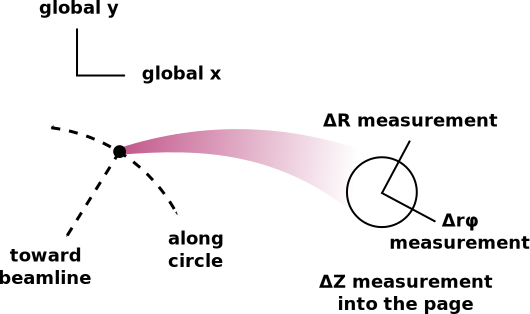
\includegraphics[width=\linewidth]{measurement.pdf}
\end{columns}

\vspace{0.25 cm}
If we had a supersector rotation of $\phi_z = 0.5$~mrad, the device would see:
\begin{itemize}
\item $\displaystyle \Delta R = \phi_z \left(Z_{\mbox{\scriptsize pos}}\right) = 0.3$~cm at end of barrel
\item $\displaystyle \Delta r\phi = 0$ \hfill (for all $R_{\mbox{\scriptsize pos}}$, $\phi_{\mbox{\scriptsize pos}}$, $Z_{\mbox{\scriptsize pos}}$\ldots\ completely insensitive)
\item $\displaystyle \Delta Z = \phi_z \left(\frac{2\pi R_{\mbox{\scriptsize pos}}}{6}\right) = 0.2$~cm at station 1
\end{itemize}
in agreement with intuition.  Is that consistent with current measurements?  What are the current measurements?
\end{frame}

\begin{frame}
\frametitle{Searching for weak modes}
\begin{itemize}
\item Another question: even if the measurements are sensitive to a
  simple supersector rotation, could it be masked by other degrees of freedom?
\item Answer: no, not for any $\phi$-symmetric deformations, at least\ldots
\end{itemize}

\vfill
\textcolor{darkblue}{\Large Method}
\begin{itemize}
\item In addition to the twist angle, allow three more degrees of
  freedom:
\begin{itemize}
\item the other two rotation angles $\phi_x$, $\phi_y$ and a radial displacement $r$ of each supersector
\item all supersectors get the same angle/displacement (that's why we're limited to $\phi$-symmetric cases)
\end{itemize}
\item Fix supersector rotation $\phi_z = 0$ or $0.5$~mrad, allow other degrees of freedom to float in Minuit
\item Minimize $(\Delta R)^2 + (\Delta r\phi)^2 + (\Delta Z)^2$
\end{itemize}
\end{frame}

\begin{frame}
\frametitle{Results}
\begin{itemize}
\item With or without $\phi_z$ fixed at 0.5~mrad, $(\phi_x, \phi_y, r)$ \mbox{minimize to $(0, 0, 0)$\hspace{-1 cm}}
\item Correlation ($\mbox{Corr}_{ij} = \mbox{Cov}_{ij} /
  \sqrt{\mbox{Cov}_{ii} \mbox{Cov}_{jj}}$) of $(r, \textcolor{darkblue}{\phi_z}, \phi_y, \phi_x)$
  has negligible off-diagonal terms:

$\displaystyle \left(\begin{array}{c c c c}
1 & \textcolor{darkblue}{-2\times 10^{-5}} & -5\times 10^{-5} & 0.0002 \\
\textcolor{darkblue}{-2\times 10^{-5}} & \textcolor{darkblue}{1} & \textcolor{darkblue}{-3\times 10^{-10}} & \textcolor{darkblue}{2\times 10^{-8}} \\
-5\times 10^{-5} & \textcolor{darkblue}{-3\times 10^{-10}} & 1 & -4\times 10^{-9} \\
0.0002 & \textcolor{darkblue}{2\times 10^{-8}} & -4\times 10^{-9} & 1 \end{array}\right) $

so these degrees of freedom are nearly independent of one another

($\textcolor{darkblue}{\phi_z}$ is the supersector twist angle)

\item Dropping terms in the $\chi^2$ (that is, assuming that the
  devices only measure one or two coordinates, not all three) leads to
  insensitivity for some parameters, but not hiding of the supersector
  rotation
\begin{itemize}
\item that is, we don't get a bad $\chi^2$ with $\phi_x$, $\phi_y$, or
  $r$ fixed to zero that is recovered when they're allowed to float
\item again, they seem to be highly independent of one another in this model
\end{itemize}
\end{itemize}
\end{frame}

\begin{frame}
\frametitle{Conclusions}
\begin{itemize}
\item Toy MC of rigid supersectors
\begin{itemize}
\item quantitatively confirmed intuition about expected residuals trends
\item allowed for a semi-systematic search for weak modes (only considered $\phi$-symmetric modes)
\end{itemize}

\item The system is fairly simple, characterized by measurement
  resolution in $\Delta R$, $\Delta r\phi$, $\Delta Z$
\begin{itemize}
\item supersector rotation model is constrained only by $\Delta R$, $\Delta Z$
\item if either is measured with better than 2--3~mm, then the model
  is well-constrained
\item it can't hide in any $\phi$-symmetric weak modes: the $\Delta
  R$, $\Delta Z$ resolutions directly determine the constraint
\end{itemize}

\item If there are significant misalignments inside the supersectors
  (as track-based residuals seem to indicate), then this model doesn't apply
\end{itemize}
\label{numpages}
\end{frame}

%% \begin{frame}
%% \frametitle{Outline}
%% \begin{itemize}\setlength{\itemsep}{0.75 cm}
%% \item 
%% \end{itemize}
%% %% \hspace{-0.83 cm} \textcolor{darkblue}{\Large Outline2}
%% \end{frame}

%% \section*{First section}
%% \begin{frame}
%% \begin{center}
%% \Huge \textcolor{blue}{First section}
%% \end{center}
%% \end{frame}

%% \begin{frame}
%% \end{frame}

\end{document}
